\subsection{\green{World model}}

In the realm of cognitive science, the concept of Bayesian cognition presents a transformative understanding of how the human brain perceives, interprets, and interacts with reality.
Tenenbaum et al. invite us to think of an analogy \cite{Ullman_Spelke_Battaglia_Tenenbaum_2017, Lake_Ullman_Tenenbaum_Gershman_2017, rule_child_2020}.
Imagine your brain as a sophisticated interactive video game engine. Just as a game engine generates dynamic virtual environments, complete with rules and physics that players interact with, the brain constructs a model of the real world. This model includes rules (physical laws, social norms), entities (objects, people), and interactions (how things work and relate to each other). We learn to navigate and predict our environment, constantly updating our internal model based on new experiences and information.
This conceptualization extends beyond mere perception, encompassing imagination, dreams, and memory. Each of these cognitive functions can be seen as manifestations of the brain's ability to generate, manipulate, and explore various scenarios and possibilities within its internal model. Dreams and imaginative constructs, while seemingly detached from reality, are composed of the same 'material' as our waking perceptions – they are all products of the brain's intricate simulation capabilities. [sources]
The self, in this view, becomes both a creator and a perceiver of its subjective reality, a reality that, while grounded in the external world, is ultimately shaped by the mind's interpretative and predictive faculties.

This paradigm posits that the brain is not merely a passive recipient of sensory inputs but rather an active participant in the construction of reality. Through the lens of Bayesian inference, the brain is conceptualized as a predictive machine. It constantly generates hypotheses or predictions about the world, drawing on past experiences and current sensory data. The brain, rather than simply processing incoming sensory information, actively infers probable causal factors behind this data, effectively reverse-engineering the world. This inferential process is guided by Bayesian principles, where the brain weighs the likelihood of various hypotheses against the evidence presented by sensory inputs. The 'prediction error' – the discrepancy between these predictions and actual sensory experiences – becomes a crucial component, informing and refining the brain's model of the world. This is the premise of many Bayesian cognitive models such as the Free-Energy. Principle, (Hierarchical) Predictive Coding, Bayesian Brain Theory, and many other variants \cite{friston_free-energy_2010, friston_world_2021} [include more sources].
The concept of the 'game engine in the head' aptly encapsulates this process, suggesting that our cognitive system operates similarly to a simulation engine, continuously constructing and updating our mental representation of the world.


\todo[inline]{Talk about intuitive physics and intuitive psychology or other research of human capabilities?}

\begin{itemize}
    \item Intuitive physics etc.
\end{itemize}

\subsection{\green{Bayesian Model}}

The fundamental tenet of Bayesian computational cognition is that the brain interprets the world by forming probabilistic models and updates them according to Bayesian inference principles. This means the brain weighs prior beliefs (previous experiences and knowledge) and the likelihood of new sensory evidence to arrive at posterior beliefs (updated model of the world). The brain uses these posterior beliefs to make predictions about future events, thus enabling adaptive behavior.
Bayesian inference can be formalized by:
\begin{equation}\label{form:bayes}
    P(z \vert x) = \frac{P(x \vert z) \cdot P(z)}{P(x)}    
\end{equation}

Where:
% \begin{conditions*}

% \end{conditions*}
    

\begin{itemize}
    \item \( P(z \vert x) \) is the posterior probability of hypothesis or latent variable \( z \) given the observed data \( x \).
    \item \( P(x \vert z) \) is the likelihood of data \( x \) given that hypothesis \( z \) is true.
    \item \( P(z) \) is the prior probability of hypothesis \( z \).
    \item \( P(x) \) is the marginal likelihood, the probability of the data \( x \).
\end{itemize}


\subsection{\green{Compositionality}}
Humans possess a native capacity for meta-cognitive evaluation, instinctively gauging the reliability of their own knowledge \cite{Lake_Ullman_Tenenbaum_Gershman_2017}. Such self-assessment serves as a compass for learning, steering the acquisition of new information in a manner that refines and optimizes our cognitive architectures.
Compositionality is central to cognitive productivity and learning. It allows for the creation of infinitely varied representations from a finite set of basic elements, similar to the mind's capacity to think an endless array of thoughts or generate countless sentences. This is particularly useful in forming hierarchical structures that simplify complex relationships, thus making inductive reasoning more efficient.
In Bayesian terms, this means that the latent $z$ can be compositional and take the form of a nested hierarchical structure.


\todo[inline]{should holarchies go here?}

\subsection{\green{Causal Models}}
Humans are endowed with an intuitive grasp of causality, which functions as the underpinning for both predictive and counterfactual reasoning \cite{Lake_Ullman_Tenenbaum_Gershman_2017}. This enables humans to extrapolate beyond the confines of empirical data, to conjure hypothetical worlds e.g. in imagination, play, and dreaming.
A causal model typically consists of a set of variables and a set of directed edges between these variables, often represented as a Directed Acyclic Graph (DAG). The vertices in this graph denote variables, which, in this context, could be seen as cognitive states. The directed edges signify causal relationships, pointing from cause to effect.
Causal models facilitate interventions, counterfactuals, and causal inference. Intervention is the ability to model the outcome of purposeful changes, represented mathematically as "do" operations  \cite{Pearl_2018}. For example, if one were to intervene to set $X = x$, the model would enable us to compute the distribution over $Y$ post-intervention.
Counterfactual reasoning allows us to traverse back in time, in a sense, and assess alternative realities — what would have happened to $Y$ if $X$ had been different?
Pearl sees this faculty as a crucial component of human cognition \cite{Pearl_2018}.



\subsection{\green{Abduction}}
How do we come up with the best explanation given partial information and limited resources? This is the problem of abduction, which can be seen as a collective term to both the generation of hypotheses, in which case it is termed \textit{abduction proper}, as well as the justification of hypotheses, also termed \textit{Inference to the Best Explanation (IBE)} \cite{burks1946peirce}.
The main problem associated with abduction proper is the difficulty of assessing how one generates fitting hypotheses quickly, while ignoring all possible non-sensical hypotheses.
Inference to the Best Explanation entails: given that we already have a set of candidate hypotheses, how do we pick the best one? Furthermore, how do we define "best"? Kwisthout presents a computational model in which he characterises "best" as an explanation that maximizes both probability as well as information content while being parsimonious \cite{kwisthout2013most}.

In the Bayesian framework the marginalisation term \( P(x) \) represents the probability of the observed data, and calculating it requires integrating over all possible hypotheses. In practical terms, this means considering how each potential hypothesis might account for every piece of observed data. This is intractable. To manage this challenge, Bayesian approximation methods provide ways to approximate \( P(x) \) without needing to perform exhaustive calculations. One common approach is to use sampling methods, such as Monte Carlo methods, which estimate 
\( P(x) \) by taking random samples from the probability distributions of the hypotheses. Another approach is variational inference, which approximates the probability distributions with simpler ones that are easier to compute. [sources + for a detailed discussion see section x]. 

It is common to divide between the generative model and the recognition density.
In this Bayesian framework, the joint probability \( P(z, x) = P(x \vert z) \cdot P(z) \) is referred to as the generative model that hypothesizes how sensory data are generated by the hidden states of the world \cite{Ramstead_Kirchhoff_Friston_2020}. In other words, it specifies a joint probability distribution over sensory inputs and potential causes of those inputs. These causes can be anything from the presence of objects in the environment to more abstract concepts like social cues.
The recognition model is an approximation of the posterior \(Q(z \vert x) \approx P(z \vert x) \), the brain's inference about the state of the world given the data.

\subsection{\green{System 1 \& System 2}}
Kahneman describes two distinct systems that characterize the dual aspects of human cognition \cite{Kahneman11}:

\emph{System 1} operates automatically and quickly, with little or no effort and no sense of voluntary control. It encompasses intuitive judgments and perceptual associations — it allows for rapid, heuristic-based processing that is often subconscious.
System 1 is akin to the generative model in Bayesian inference. Just as System 1 can produce instantaneous responses and intuitions, the generative model provides immediate perceptual hypotheses and predictions that guide behavior in a fluid and dynamic manner without the need for conscious deliberation.

\emph{System 2} allocates attention to the effortful mental activities that demand it, including complex computations. It is associated with the conscious, rational mind and is deliberate, effortful, and orderly. 
The process of updating the recognition density is more reflective and can be related to the slow, controlled inference that characterizes conscious thought. Adjusting the recognition density is akin to the effortful correction or modulation of System 1's rapid predictions when errors are detected or when more complex reasoning is required.

For example, when learning to play the piano, initial efforts require conscious attention and deliberate practice to master certain phrases (System 2). Over time, as these phrases become internalized, they can be executed more automatically and intuitively (System 1). This transition illustrates how learned skills move from conscious, effortful control to intuitive, automatic execution, mirroring the interplay between the recognition density (System 2) and the generative model (System 1) in Bayesian cognition.


\subsection{\green{Concepts}}
Concepts, as the building blocks of thought, vary widely in their forms and representations. They range from concrete, perceivable objects such as 'a table' to abstract notions like 'love' or 'money', theoretical constructs ('the gene', 'the atom'), mathematical entities ('addition', 'multiplication'), and even non-existent entities like 'a unicorn'. This variety, as highlighted by Blouw et al. \cite{blouw2016concepts}, underscores the diverse spectrum of concepts that the human mind can conceive and manipulate.

An effective conceptual framework not only categorizes these varied forms but also explains their \emph{extension} (why a concept refers to certain things and not others) and \emph{intension} (why it describes these referents in specific ways) \cite{ball2013surfaces}. The concept space, therefore, must be understood as a multidimensional and dynamic entity, where concepts are not isolated but embedded in a rich tapestry of relationships and attributes.

Several key criteria help in mapping and understanding this concept space:

\begin{description}
    \item [Relationship Path] This refers to the connections between concepts, governed by their similarities, differences, and functional relationships. It explains how one concept is related to or can be derived from another.
    \item [Mutual Information] This criterion examines how well concepts predict each other, based on their co-occurrence and interaction in reality. It reflects the degree to which the presence or understanding of one concept informs about another.
    \item [Change Distance] This involves measuring the conceptual 'distance' or difference between two concepts. It accounts for the extent of transformation or cognitive shift required to move from one concept to another in the conceptual space.
    \item [Parameter Distance] This refers to the number of 'knobs' or minimal changes needed to transition from one concept to another. For example, determining the minimal edits or shifts needed to transform the concept of 'dog' to 'cat', or 'rock' music to 'jazz'. This concept is akin to edit distance in text or Kolmogorov complexity in information theory, offering a quantifiable measure of conceptual transformation.
\end{description}
[need sources for all of these]

[kiki, bobo, other examples]
% E.g. "dog" should be closer to "canine" than to "panda".


\subsection{\red{Varied Representations}}
MAP vs POST


\subsection{\green{Large Language Models}}\label{sec:llm}

% show that this allows for analogical thought and reasoning
% perhaps include bit from AAPS proposal

In his recent book "What is ChatGPT doing?", Stephen Wolfram analyses the internal mechanisms of Large Language Models (LLMs) such as GPT \cite{wolfram2023chatgpt}.
LLMs are descendents of the Transformer architecture, originally introduced in 2017 by Vaswani et al. \cite{Vaswani_Shazeer_Parmar_Uszkoreit_Jones_Gomez_Kaiser_Polosukhin_2017} and are trained on massive datasets of text and code. This allows them to learn the statistical relationships between words and phrases, and to generate human-quality text, translate languages, write different kinds of creative content, and answer questions in an informative way.
Embedding is the process of converting tokens into dense vectors of numbers. These vectors represent the semantic and syntactic information about the tokens. The embedding layer is important for LLMs because it allows them to learn the relationships between tokens in a high-dimensional space.
Various levels of embeddings are encoded, which gives aggregate words, sentences, paragraphs, etc. positions in this latent space.
LLMs primarily learn and operate through next token prediction. They use statistical patterns in data to predict language use, context, and meaning, focusing on determining the next word or phrase in a sequence. This predictive training over time leads to a complex internal representation of language, enabling the model to produce responses that are grammatically correct, contextually relevant, and semantically nuanced.
Wolfram highlights that GPT doesn't have any explicit knowledge of grammar and the parse trees that govern natural language, yet they learn these nested syntax trees implicitly. 
Nonsense sentences such as Chomsky's famous example "Colorless green ideas sleep furiously" [source], or jabberwocky sentences [source], show that there is more to language than syntax. There seems to be a semantic grammar, which LLM models learn implicitly.
LLMs, through exposure to vast amounts of text containing conditional and logical structures (e.g., "if X, then Y"), develop an ability to recognize and generate logically coherent sentences. They seem to mimic forms of syllogistic reasoning, as seen in sentences like "All X are Y. This is not Y, so it's not X." (as in "All giraffes are tall. This is not tall, so it's not a giraffe."). 
It's possible that LLMs have "discovered" syllogistic logic by looking at huge amounts of text. However, when it comes to more sophisticated formal logic, they fail [source], since they learned this implicit logic by correlation and they don't "know" the actual rules of logic.
The concept space that LLMs navigate can be illustrated through analogies such as "man is to king as woman is to queen." This represents the learnt semantic space, where relationships and associations are encoded in a high-dimensional embedding space. In this space, concepts and words are positioned in such a way that their relative distances and directions encode meaningful relationships, mirroring the complexities of human language and thought.


\begin{figure}
    \centering
    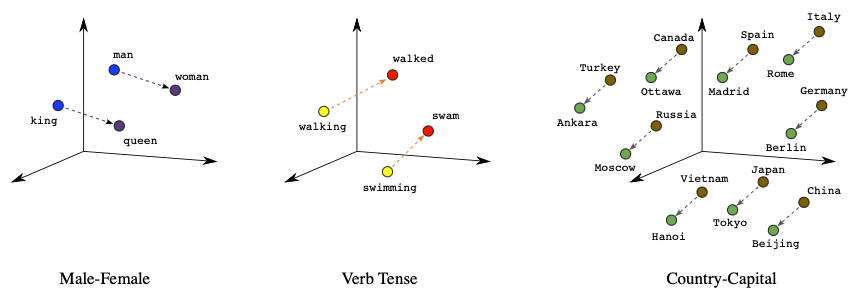
\includegraphics[width=\textwidth]{../img/embeddings_analogies.png}
    \caption{taken from google}
    \label{}
\end{figure}






- holarchic direction sensory data to features, etc. 






\subsection{\green{Probabilistic Programming}}

Dehaene et al. posit that human cognition is uniquely characterized by its ability to form symbolic representations and recursive mental structures akin to a language of thought, enabling the creation of domain-specific conceptual systems \cite{dehaene_symbols_2022}. This cognitive ability allows for the generation of new concepts through the compositional arrangement of existing elements, a process exemplified by the derivation of geometric concepts. Cognition simplifies complex patterns into mental representations via mental compression, where the complexity of a concept is measured by the length of its mental representation as per the Minimum Description Length (MDL) principle.

Neuroscientific research indicates the presence of specialized brain circuits responsible for processing different domains of these languages of thought, with certain brain regions involved in linguistic processing and others in non-linguistic domains like mathematics and spatial reasoning [source]. The recognition of mathematical patterns is linked to the ability to detect repetition with variation, a process underpinned by specific neural areas that vary with cognitive domain.

\begin{figure}[H]
    \centering
    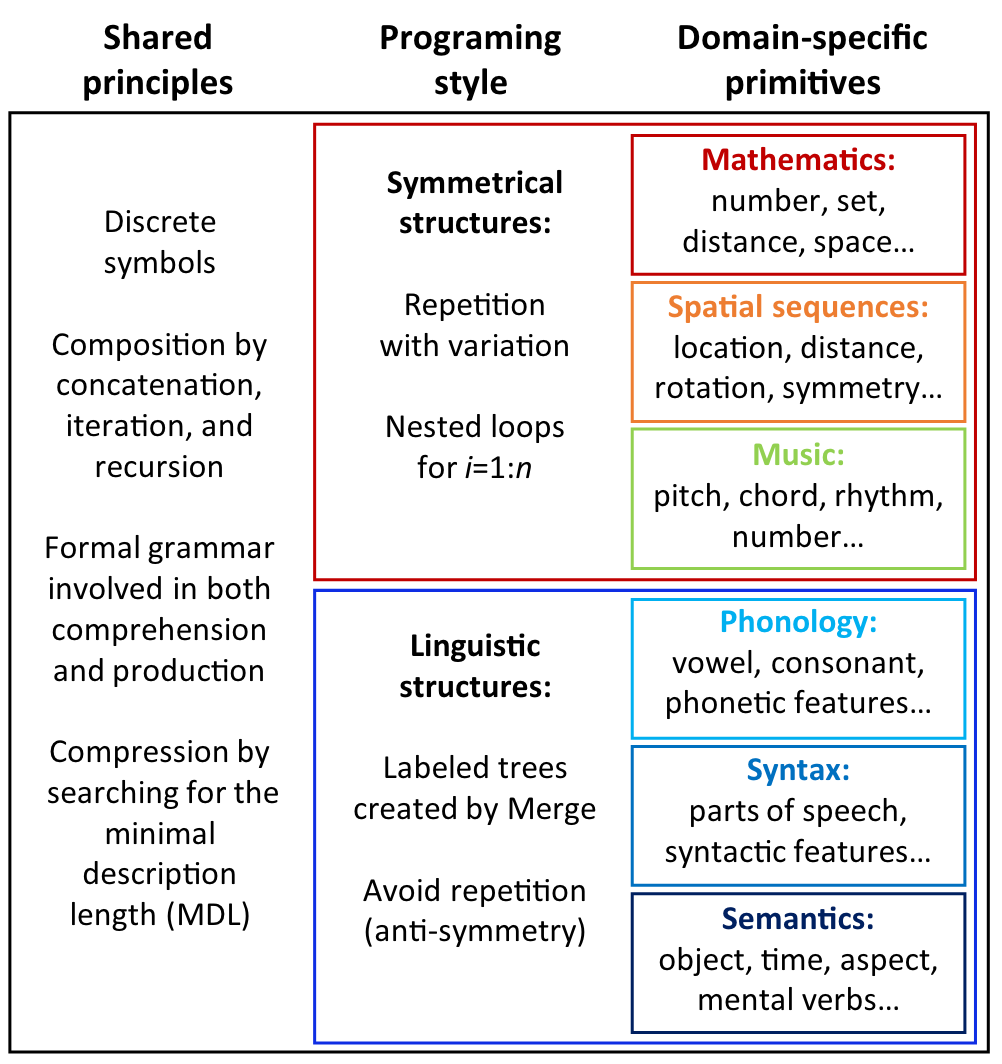
\includegraphics[width=0.7\textwidth]{../img/DSL.png}
    \caption{image taken from \cite{dehaene_symbols_2022}}
    \label{fig:DSL}
\end{figure}

Distinct from other primates, humans have developed the capability to use symbols in complex, rule-based systems, highlighting a unique aspect of human cognitive development. Non-human primates may associate signs with concepts; however, they do not appear to use these in the recursive, rule-based manner that humans do.

[Tenenbaum et al] posit that the brain implements mechanisms analogous to those found in probabilistic programming languages, enabling it to represent and infer the probabilistic structure of the world. Probabilistic programming provides a framework for defining complex probabilistic models and for performing inference in these models, and the hypothesis is that the brain engages in similar computational processes. [multiple sources]

Experiments show that humans do not seem to start from blank-slate but rather from rich domain knowledge [argument for primitives, more sources] \cite{lake_building_2016}. Lake et al. propose that concepts can be represented as simple stochastic programs [elaborate]. A program here can be thought of a procedure that generates more examples of the same concept. If a program would represent the concept "animal", if would generate examples such as "giraffe", "zebra", "fish", and so on. Of course, higher-level programs could produce lower-level programs, in other words, in this paradigm, the essential aspect of compositionality gives rise to a part-whole hierarchical structure, i.e. a holarchy [reference].

% The idea is that we model the world by creating programs that generate our observations \cite{rule_child_2020}.


% Roumi et al.'s experiment indeed suggest that humans may interpret and compress sequence regularities in a type of program of minimum description length (MDL) \cite{al_roumi_mental_2021}.
% Dehaene et al. further test this hypothesis and find similar results \cite{dehaene_symbols_2022}.


[the assumption we make here is that features are somehow aggregated or extracted into symbols [see \cite{garcez_neurosymbolic_2020}], primitives, along with possibly innate symbols \cite{Lake_Ullman_Tenenbaum_Gershman_2017}] 


% \subsection{\red{review of human capabilities and comparing PPL vs LLMs}}

% \subsubsection{\red{World Model}}
% \subsubsection{\red{Bayesian Model}}
% \subsubsection{\red{Compositionality}}
% \subsubsection{\orange{Causality}}
% \subsubsection{\red{Correlation Does Not Imply Causation}}

% Generative models assign probability distributions, representing observations in such a way that they can generate new data points similar to the observations. The mapping between the probability distributions and the data is correlational. 

% Causal models in contrast, represent hypotheses of how observations were generated. They do not just represent the observations by correlation, but aim to accurately reflect the mechanisms by which the data originated.[source]



% [The Reichenbach Principle, named after philosopher Hans Reichenbach, is a foundational concept in the philosophy of science, particularly in the study of causation. It essentially states that if two events are found to be statistically correlated, then there must exist some causal connection between them. This causal connection can manifest in three forms: either one event causes the other, the second event causes the first, or both events are influenced by a common cause. This principle highlights the difference between mere correlation (statistical association) and causation (a direct or indirect relationship leading to the occurrence of an event).

% The significance of the Reichenbach Principle becomes clear when considering why causal models contain more information than purely statistical ones. Statistical models excel at identifying and quantifying relationships between variables based on observed data. They can tell us, for example, that two variables tend to vary together in a predictable way. However, statistical models don't inherently provide information about the directionality or the underlying mechanism of these relationships – they don't tell us whether one variable causes changes in the other, or if both are influenced by an external factor.

% Causal models, in contrast, are designed to map out these directional relationships. They go beyond mere association to explain how one variable affects another. This is done by incorporating knowledge of the underlying mechanisms and processes that drive the relationships between variables. In a causal model, variables are not just connected; they are linked in a way that specifies how changes in one will lead to changes in another.

% For example, consider the relationship between smoking and lung cancer. A statistical model can show that smoking is correlated with an increased risk of lung cancer, but it doesn't explain why this is the case. A causal model, on the other hand, can illustrate how smoking leads to biological changes in the body that increase the risk of developing lung cancer, thereby providing a more comprehensive understanding of the relationship.

% In summary, the Reichenbach Principle underscores the necessity of seeking causal explanations behind observed correlations. While statistical models are powerful tools for identifying patterns and relationships in data, causal models offer a deeper level of understanding. They provide insights into the mechanisms and processes underlying these patterns, allowing for more accurate predictions, effective interventions, and a richer comprehension of the phenomena being studied.]
% \cite{causal_representation_learning}
% \subsubsection{\red{Abduction}}
% \subsubsection{\red{System 1 \& 2}}
% \subsubsection{\red{Concepts}}

% \rephrase[inline]{from JB: LLMs learn how to complete sequences, they do statistics over patterns}
% Stephen shows that when LLMs create statistics over text, they first discover patterns, then syntax, then style, and only lastly semantics. Humans however start out by discovering semantics and then find patterns, syntax and lastly style. 



% - Can LLMs extract composable entities to recombine?

% % PROS:
% % - Semantics vs Syntax, semantic grammar
% % - vector representations of concepts, vector algebra, distance, etc. 
% % - Compositionality


% % CONS:
% % - They conflate an implicit world model with inference. (model in wolframs terms)
% % - they lack causality.
% % - pattern to syntax etc. vs other way around



% \begin{itemize}
%     \item could LLMs be regarded as symbolic like models? since each token is a vector and then the model builds aggregate representations given those vectors?
% \end{itemize}



% \begin{table}
%     \centering
%     \begin{tabular}{|l|c|c|}
%         \hline
%         \textbf{Aspects of cognition} & \textbf{LLMs} & \textbf{PPL} \\\hline
%         Compositionality & $\times$ & $\checkmark$ \\\hline
%         System 1 \& 2    &          & \\\hline
%         Causality        & $\times$ & $\checkmark$ \\\hline
%         Analogy          &          & \\\hline
%         Abduction        &          & \\\hline
%         Symbolic Reasoning & $\times$ & $\checkmark$ \\\hline
        
%     \end{tabular}
%     \caption{title}
%     \label{}
% \end{table}


